\subsection{Blockchain}
% 
Since the inception of a digital currency Bitcoin (described in the following section) in 2009, blockchain has been part of the discussions about this novel approach to currency. Over the time, the perception shifted from seeing blockchain just as a part of cryptocurrency into seeing it as an separate, innovative, even disruptive technology. Some media mark \textit{blockchain} to be the word of the year 2017\footnotemark, while others comparable it to inception of the Web in 1990s~\cite[p. 14]{Swan2015BlockchainEconomy}.
% 
\footnotetext{\url{https://www.theguardian.com/technology/2018/jan/30/blockchain-buzzword-hype-open-source-ledger-bitcoin}, accessed 28-03-2018}

From the perspective of cryptocurrency, blockchain is a public ledger, that contains all the transactions of the cryptocurrency to date~\cite{Swan2015BlockchainEconomy}. It is distributed among all the computers participating in the consensus process. Since it contains all the past transactions (since the inception of the currency), data is never deleted from the blockchain. All changes happen only as amendments to the latest version of the blockchain. A \textit{change} could be virtually any data. For example, it could be details of latest transactions (as is the case with Bitcoin) or newly deposited agreements (as in Quorum - enterprise level ledger\footnotemark). This \textit{change} is called a \textit{block}. Blocks are the fundamental parts, that make up the blockchain. When a new blockchain is created, a first set of changes becomes the first block.
% 
\footnotetext{Quorum is a blockchain-based private storage for agreements. Its intended users are enterprises in the finance industry, who are trading financial derivatives and who need to reach an agreement, while maintaining acceptable level of privacy.
\begin{flushleft}
\url{http://fortune.com/2016/10/04/jp-morgan-chase-blockchain-ethereum-quorum/}, accessed 28-03-18
\url{https://www.jpmorgan.com/global/Quorum}, accessed 28-03-18
\end{flushleft}
}
% 
When more changes are made (for example, more transactions are processed), a new block is created. The creation of a new block involves computing a hash value of the previous block. This hash value is then included in the new block, together with the data comprising the change. By including the hash value of the old block in the new block, these two blocks are now linked. All the blocks in the blockchain are linked together in such fashion. Figure~\ref{fig:blockch-basics} illustrates this principle. 
% 
\begin{figure}[ht]
    \centering
    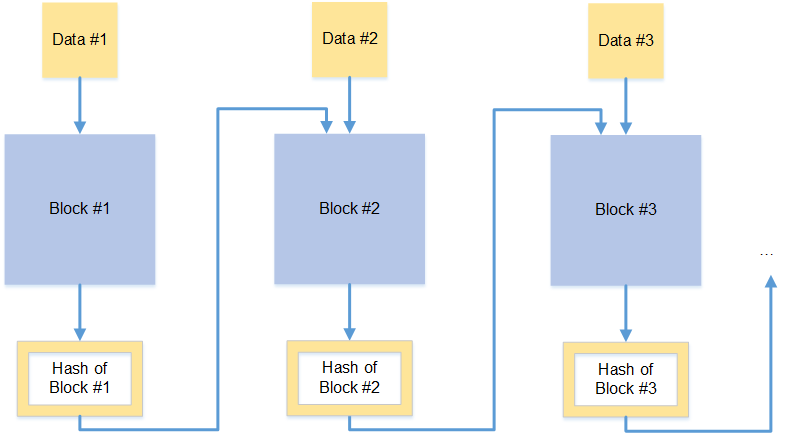
\includegraphics[width=.95\textwidth]{blockchain-basics}
    \caption{The basic architecture of a blockchain. If Block \#1 is the first block in the chain, it is also referred to as the \textit{genesis block}.}
    \label{fig:blockch-basics}
\end{figure}

It is not possible to alter the past blocks in the blockchain. In order to accomplish this, we would need to find such a combination of data, that would produce the same hash. This violates the pre-image resistance property of the hash function. Alternative technique could be to change the data in block \textit{n}, then calculate new hash and include it in block \textit{n+1} and so on, recalculating every subsequent block~\cite[3]{NakamotoBitcoin:System}. The decentralisation of the blockchain prevents this. Every participating node maintains and updates its own copy of the blockchain. When there is a dispute about the correct version of the blockchain, the version that is present on most nodes is chosen as the correct one and the other versions are discarded. Therefore, an attacker would need to control the majority of the nodes in the network in order to include counterfeit data in the blockchain. If it is not possible to determine, which version of the blockchain is present on more nodes, the blockchain \textit{forks}. This means, that some nodes will continue building up on one version of the blockchain, while other nodes will continue building up on another version. The version of the blockchain that is the first one to receive next calculated block we then become the correct one. References to the other (incorrect) version are part of the blockchain in some systems (e.g. in Ethereum the other versions of the blockchain are called \textit{uncles} and their hash needs to be included in the newly calculated block) and discarded in other systems (e.g. in Bitcoin).

The possibility of temporary blockchain forks due to two nodes calculating a valid block at the same time gives importance to the concept of a \textit{transaction confirmation}. A transaction confirmation means, that a valid block was calculated on top of the block with the transaction. The number of required confirmations, before a transaction is considered valid, varies by the system (e.g. 6 confirmations are considered sufficient in Bitcoin), but in general, more confirmations mean higher certainty that the transaction is valid\footnotemark.
% 
\footnotetext{\url{https://en.bitcoin.it/wiki/Confirmation}, accessed 18-05-2018}

Based on the use of the blockchain, three `levels' can be identified~\cite{Swan2015BlockchainEconomy}:
\begin{itemize}[noitemsep, nolistsep]
    \item \textit{Level 1} is blockchain used with currency only. The data here are transactions of that currency. Level 1 of blockchain would be for example Bitcoin.
    \item \textit{Level 2} includes smart contracts and more advanced transactions and agreements than Level 1. However, Level 2 of blockchain is still tied to financial applications in some way. Example of Level 2 blockchain is Ethereum platform.
    \item \textit{Level 3} of blockchain includes usage outside of financial applications, in sectors such as government or health-care~\cite{Swan2015BlockchainEconomy}.
\end{itemize}

% Motivate problems with cryptocurrency? Double spending problem and byzantines general problem? 
% Central bank system - problems?
% Decentralised system - solutions
% mentioned briefly - drawbacks
% narrower definition of blockchain - list of transactions for a cryptocurrency
% broader definition - number of other applications, Blockchain 2.0 and Blockchain 3.0 as described by Swan